\documentclass{standalone}
\usepackage{tikz}
\usepackage{tkz-graph}
\usepackage{tkz-berge}

\begin{document}

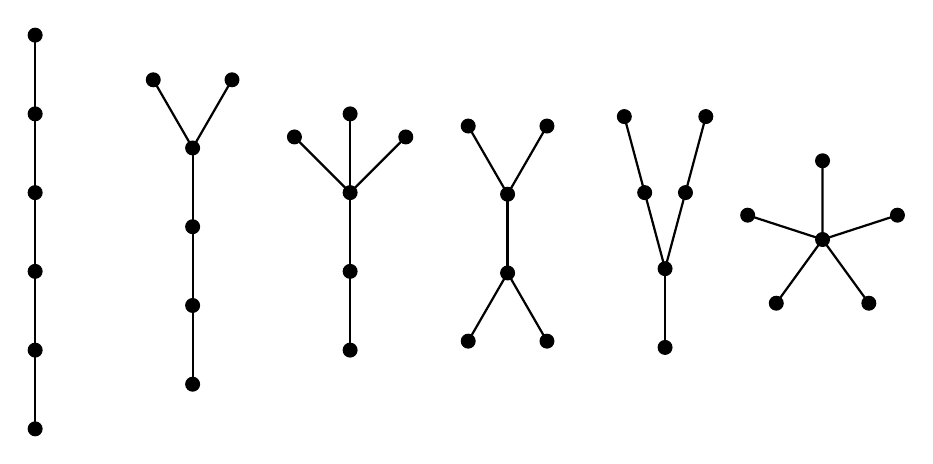
\begin{tikzpicture}

  \GraphInit[vstyle=Simple]
  \tikzset{VertexStyle/.style = {
  shape = circle,
  fill = black,
  inner sep = 0pt,
  outer sep = 0pt,
  minimum size = 5pt,
  draw}}

  \begin{scope}[xshift=0cm, yshift=-2.5cm]
    \Vertex[x=0, y=0]{A1};
    \NO(A1){A2};
    \NO(A2){A3};
    \NO(A3){A4};
    \NO(A4){A5};
    \NO(A5){A6};
    \Edge(A1)(A2);
    \Edge(A2)(A3);
    \Edge(A3)(A4);
    \Edge(A4)(A5);
    \Edge(A5)(A6);
  \end{scope};

  \begin{scope}[xshift=0cm, yshift=-1.933cm]
    \Vertex[x=2, y=0]{B1};
    \NO(B1){B2};
    \NO(B2){B3};
    \NO(B3){B4};
    \begin{scope}[xshift=2cm, yshift=3cm]
      \Vertex[a=90+30, d=1cm]{B5};
      \Vertex[a=90-30, d=1cm]{B6};
    \end{scope};
    \Edge(B1)(B2);
    \Edge(B2)(B3);
    \Edge(B3)(B4);
    \Edge(B4)(B5);
    \Edge(B4)(B6);
  \end{scope};

  \begin{scope}[xshift=0cm, yshift=-1.5cm]
    \Vertex[x=4, y=0]{C1};
    \NO(C1){C2};
    \NO(C2){C3};
    \NO(C3){C4};
    \begin{scope}[xshift=4cm, yshift=2cm]
      \Vertex[a=90+45, d=1cm]{C5};
      \Vertex[a=90-45, d=1cm]{C6};
    \end{scope};
    \Edge(C1)(C2);
    \Edge(C2)(C3);
    \Edge(C3)(C4);
    \Edge(C3)(C5);
    \Edge(C3)(C6);
  \end{scope};

  \begin{scope}[xshift=0cm, yshift=-1.366cm]
    \Vertex[x=6, y=0.8457]{D1};
    \begin{scope}[xshift=6cm, yshift=0.8457cm, rotate=180]
      \Vertex[a=90+30, d=1cm]{D2};
      \Vertex[a=90-30, d=1cm]{D3};
    \end{scope};
    \NO(D1){D4};
    \begin{scope}[xshift=6cm, yshift=1.8457cm]
      \Vertex[a=90+30, d=1cm]{D5};
      \Vertex[a=90-30, d=1cm]{D6};
    \end{scope};
    \Edge(D1)(D2);
    \Edge(D1)(D3);
    \Edge(D1)(D4);
    \Edge(D4)(D5);
    \Edge(D4)(D6);
  \end{scope};

  \begin{scope}[xshift=0cm, yshift=-1.4659cm]
    \Vertex[x=8, y=0]{E1};
    \NO(E1){E2};
    \begin{scope}[xshift=8cm, yshift=1cm]
      \Vertex[a=90+15, d=1cm]{E3};
      \Vertex[a=90+15, d=2cm]{E5};
      \Vertex[a=90-15, d=1cm]{E4};
      \Vertex[a=90-15, d=2cm]{E6};
    \end{scope};
    \Edge(E1)(E2);
    \Edge(E2)(E3);
    \Edge(E2)(E4);
    \Edge(E3)(E5);
    \Edge(E4)(E6);
  \end{scope};

  \begin{scope}[xshift=0cm, yshift=-0.9045cm]
    \Vertex[x=10, y=0.80901]{F1};
    \begin{scope}[xshift=10cm, yshift=0.80901cm]
      \Vertex[a=1*360/5+90, d=1cm]{F2};
      \Vertex[a=2*360/5+90, d=1cm]{F3};
      \Vertex[a=3*360/5+90, d=1cm]{F4};
      \Vertex[a=4*360/5+90, d=1cm]{F5};
      \Vertex[a=5*360/5+90, d=1cm]{F6};
    \end{scope};
    \Edge(F1)(F2);
    \Edge(F1)(F3);
    \Edge(F1)(F4);
    \Edge(F1)(F5);
    \Edge(F1)(F6);
  \end{scope};
\end{tikzpicture}

\end{document}
